\documentclass[../../master_thesis_np.tex]{subfiles}
\graphicspath{{./imgs/}}

\begin{document} 
\chapter{Introduction}
	The phenomenon of (passive) Brownian Motion is a well investigated topic in physics since 1827, when Robert Brown studied the motion of pollen grains suspended in water. The list of physicists who dealt with the topic contains names such as Einstein and Langevin \parencite{gardiner_handbook_2004}, whose main contribution is the first formalization of Brownian motion in terms of a differential equation, Ornstein and Uhlenbeck, who calculated fundamental properties such as the mean-square displacement of a Brownian particle \parencite{uhlenbeck_theory_1930}. Since then, scientists across various fields have explored the properties of Brownian Particles systems in numerous variations, one of which is Active Brownian Particles (ABP). 
	
	ABPs are distinguished by their ability to extract energy from the environment and use it to propel themselves making them a fundamental model for non-equilibrium active matter systems.	
	The motility mechanism can be mechanic, like cilia or flagella used by micro-organisms, or thermodynamic, like phoresis of various nature. 
	
	Incorporating self-propulsion within the Brownian framework enables the emergence of numerous novel behaviors, with collective dynamics being particularly noteworthy; even if the single agent details may differ, especially in propulsion mechanisms, it is possible to build minimal statistical physics models that mimic real world dynamics, leading the way to the discovery of new physics as well as methods to analyze real living beings' behaviors and new ideas in material science. 
	
	There are several model features and properties that can be exploited to develop both analysis methods and new technologies based on active matter, e.g.\ self organization and clustering are relevant in the study of bacterial and algae colonies, while in the artificial world much use can be made of properties like chaining, clustering or vortices.
	\newpage
	
	\section{Micro Scale Robotics and CELLOIDS}
	The first one to bring the concept of robotics at micro scale, especially for medical applications into a scientific context was Richard Feynman in the famous 1959 CalTech conference \citetitle{Feynman}, from which the following quote is taken:
	\begin{displayquote}
		Many of the cells are very tiny, but they are very active \omissis Consider the possibility that we too can make a thing very small which does what we want — that we can manufacture an object that maneuvers at that level!
		
		\omissis it would be interesting in surgery if you could swallow the surgeon. You put the mechanical surgeon inside the blood vessel and it goes into the heart and "looks" around. \omissis It finds out which valve is the faulty one and takes a little knife and slices it out. Other small machines might be permanently incorporated in the body to assist some inadequately functioning organ.\footcite{Feynman}
	\end{displayquote}
	
	The scaling laws of physical quantities, especially regarding friction and hydrodynamics, prevent the construction of a micrometer scale robot which is just a miniaturized version of a macroscopic one. Swimming in a fluid for the typical size and speed we are interested in-meaning, at low Reynolds number $\mathrm{Re} \equiv \frac{\rho v L}{\eta}$-is quite a different game than what we are used to in the macroscopic world. When inertia is negligible, it is impossible to swim using a \emph{reciprocal motion}, that is, a cyclic motion that follows the same path forward and back \cite{purcell_life_1977}. Needles to say that turning a propeller with a miniaturized macroscopic motor won't be optimal at this scale, since its starting torque would be extremely large. These huge difficulties are encountered if one just wants to swim in a simple fluid. Using a micro robot in real life brings some other challenges in the problem, such as swimming in viscoelastic media like hyaluronic acid lattices or shrinking through the small interstices in between living cells.
	
	One way of solving this kind of problems is through bio-inspiration: tackling challenges by mimicking the gimmicks nature uses to overcome them. The aim of CELLOIDS, the project inside of which this work has taken place, is to build a micro-scale intelligent robotic system that takes inspiration from the amoeboid propulsion of immune cells. The CELLOIDS’ concept for a microrobot is a phospholipids GUV (Giant Unilamellar Vesicle) filled with a suspension of ABPs. A single ABP is a Janus sphere, with an inert hemisphere and a catalytic one, which turns a fuel into some products generating a gradient in the concentration field in its vicinity; this makes the solvent flow around the particle causing it to move. In particular, the most studied Janus Sphere in this field is a \ch{SiO2} sphere where \ch{Pt} is deposed using some techniques to coat just one hemisphere; the fuel is \ch{H2O2} that is decomposed in 
	\begin{align}
		\ch{2 H2O2 ->[Pt] 2 H2O + O2}
	\end{align}
	using platinum as catalyst.
	
	The GUV’s walls are deformable and can be pushed from the inside by ABPs, leading to further deformation and, in the end, motility, mimicking the behavior of living cells that can shrink through the tiny interstices of a biological tissue.
	
	\section{Objectives}	
	In the previously described framework, collective behaviors and emergent properties of ABPs systems, both self-induced and caused by the interaction with a rigid or deformable confinement are of paramount importance for the microrobot to work properly. Regarding the self-induced behaviors, the most investigated is Motility-Induced Phase Separation \parencite{cates_motility-induced_2015}, caused by the concurrence between the excluded volume of the particles (non superimposable hard spheres) and their activity. A confinement-induced emergent property is e.g.~propulsion-induced accumulation, in which motile particles tend to cluster at the boundary of the confinement \parencite{marconi_towards_2015}.
	
	The objective of this work is to develop a model, a simulation framework and a suite of analysis tools to study how an explicit interaction potential changes single and collective behaviors of an ABP system, always keeping in mind the experimental and applied point of view. The main novelty in the model is how a potential is applied. Specialized literature focuses on two types of interactions: aligning, involving the direction of particles, and non-aligning, which can be simple central potentials like a hard sphere excluded volume interaction; it is possible to find several interactions of both types in literature but this work tries to unify the two, linking coupling between the positions of a pair of particles (force) with coupling between the orientations of said particles (torque) with the objective of developing a minimal model that tries to mimic experimental observations.
	
	Here, the term \emph{minimal} means not only that a unique interaction potentials is used to couple both positional and orientational degrees of freedom, but also that this simple model could be enough to simulate real world phenomena without looking into the hydrodynamics, which will involve simulating not only the particles but the solvent as well, leading to extremely heavy simulations. Moreover, details about how the solvent flows around a phoretic ABP, as well as the concentration field around it, are still a matter of investigation and have been simulated mostly for single particles. Here, we preferred to stick with dry active matter modeling.
	
	Given this novel modeling technique and its implementation, the next step of this work is to obtain a qualitative, eyesight agreement between simulations and experiments, making the \emph{in silico} experiment able to capture all the features and dynamics observed \emph{in vitro} scanning the different parameters.
	
	Moreover, with the right parameters, this model is capable of showing rich collective behaviors, making it a feasible alternative to study phase transitions in a statistical physics fashion. A glorious model in this field involving aligning interactions is the Vicsek model \parencite{vicsek_novel_1995}, which captures a plethora of natural world phenomena. Present work shows how a system with coupled positions and orientations can turn into a continuous Vicsek-like case study.
	
	The last objective of the project is to build a Deep Learning based tool which, when trained starting from a minimal set of simulation data, is able to infer the interaction potential between couples of particles both in simulated and experimentally observed situations.
	
	
	\section{Literature and State of the Art}
	
	Active matter is a lively field and plenty of literature has been produced on the topic. We will go through some of the  different papers that tackle the problem of understanding how active Brownian particles, both single and systems, behave with and without interactions.
	
	\subsection{Collective motion}
	Investigation of collective motion is an extremely important topic in this field, since it not only lead to a better understanding of the physics behind ABPs systems, but it helped developing physical and mathematical tools such as order parameters which can be used both in simulation and experimental context. 
	
	In the following section the Vicsek model will often be cited. This is the right time to give a brief introduction to it with the authors' words:
	 \begin{displayquote}
		The only rule of the model is: at each time step a given particle driven with a constant absolute velocity assumes the average direction of motion of the particles in its neighborhood of radius r with some random perturbation added.\footcite{vicsek_novel_1995}
	 \end{displayquote}
	 Although extremely simple, this model is of paramount importance in the study of active matter since it can be studied in terms of a phase transition and recreates in some way the behavior of real living systems.
	
	Although not strictly related with present work,\parencite{cavagna_empirical_2010, ballerini_interaction_2008} are essential papers for the study of collective motion, for the problem of relating theoretical models and reality is tackled analyzing data of starling swarms in order to understand characteristics of interactions. Understandably, the system studied by \citeauthor{cavagna_empirical_2010, ballerini_interaction_2008} is pretty different from the active Brownian particles ensemble investigated in this project, with the fist difference being the dimensionality (a bird swarm, just like a school of fish moves in a 3D environment), but some of the problems reported in that paper are still present in these days active matter community.
	
	The next few papers focus on systems which are more akin to what will be investigated from chapter~\ref{chap:int_impl} on. \parencite{martin-gomez_collective_2018} analyzes how an explicit polar aligning interaction can make the system transition to an ordered flocking phase, where almost all particles align their orientation in the same direction, even though an orientational noise is present. The model is built taking into account an aligning torque between particles $i$ and $j$ which goes as $K \sin{(\theta_{i} - \theta_{j})}$, only within a certain distance, and a repulsive potential $\epsilon \left(\frac{\sigma}{r}\right)^{12}$ to take into account the excluded volume.
	
	The parameters of the system are the Péclet number $\mathrm{Pe} = \frac{v_0}{\sigma \gamma}$ which is the ratio between the self propulsion velocity and the product of the characteristic length of the particles and the rotational diffusion coefficient and $g = \frac{K}{4\pi \sigma^2 \gamma}$ which quantifies the relative intensity of the orientational coupling strength and the reorienting noise. The order parameter is the mean global polarization
	
   	\[ P = \frac{1}{N}\left| \sum_{k=1}^{N} \exp{(i \theta_k(t))} \right|\]
  	 which is $\sim 0$ in the disordered phase and $> 0$ in the flocking phase. The authors build a phase diagram in the $\mathrm{Pe}-g$ plane Figure \ref{fig:martin_flocking1}, which shows the separation between disorder and flocking as well as intermediate clustering phases, one with a microscopic cluster structure and one where a macroscopic single cluster structure arises.
	
	\begin{figure}[h]
		\centering
		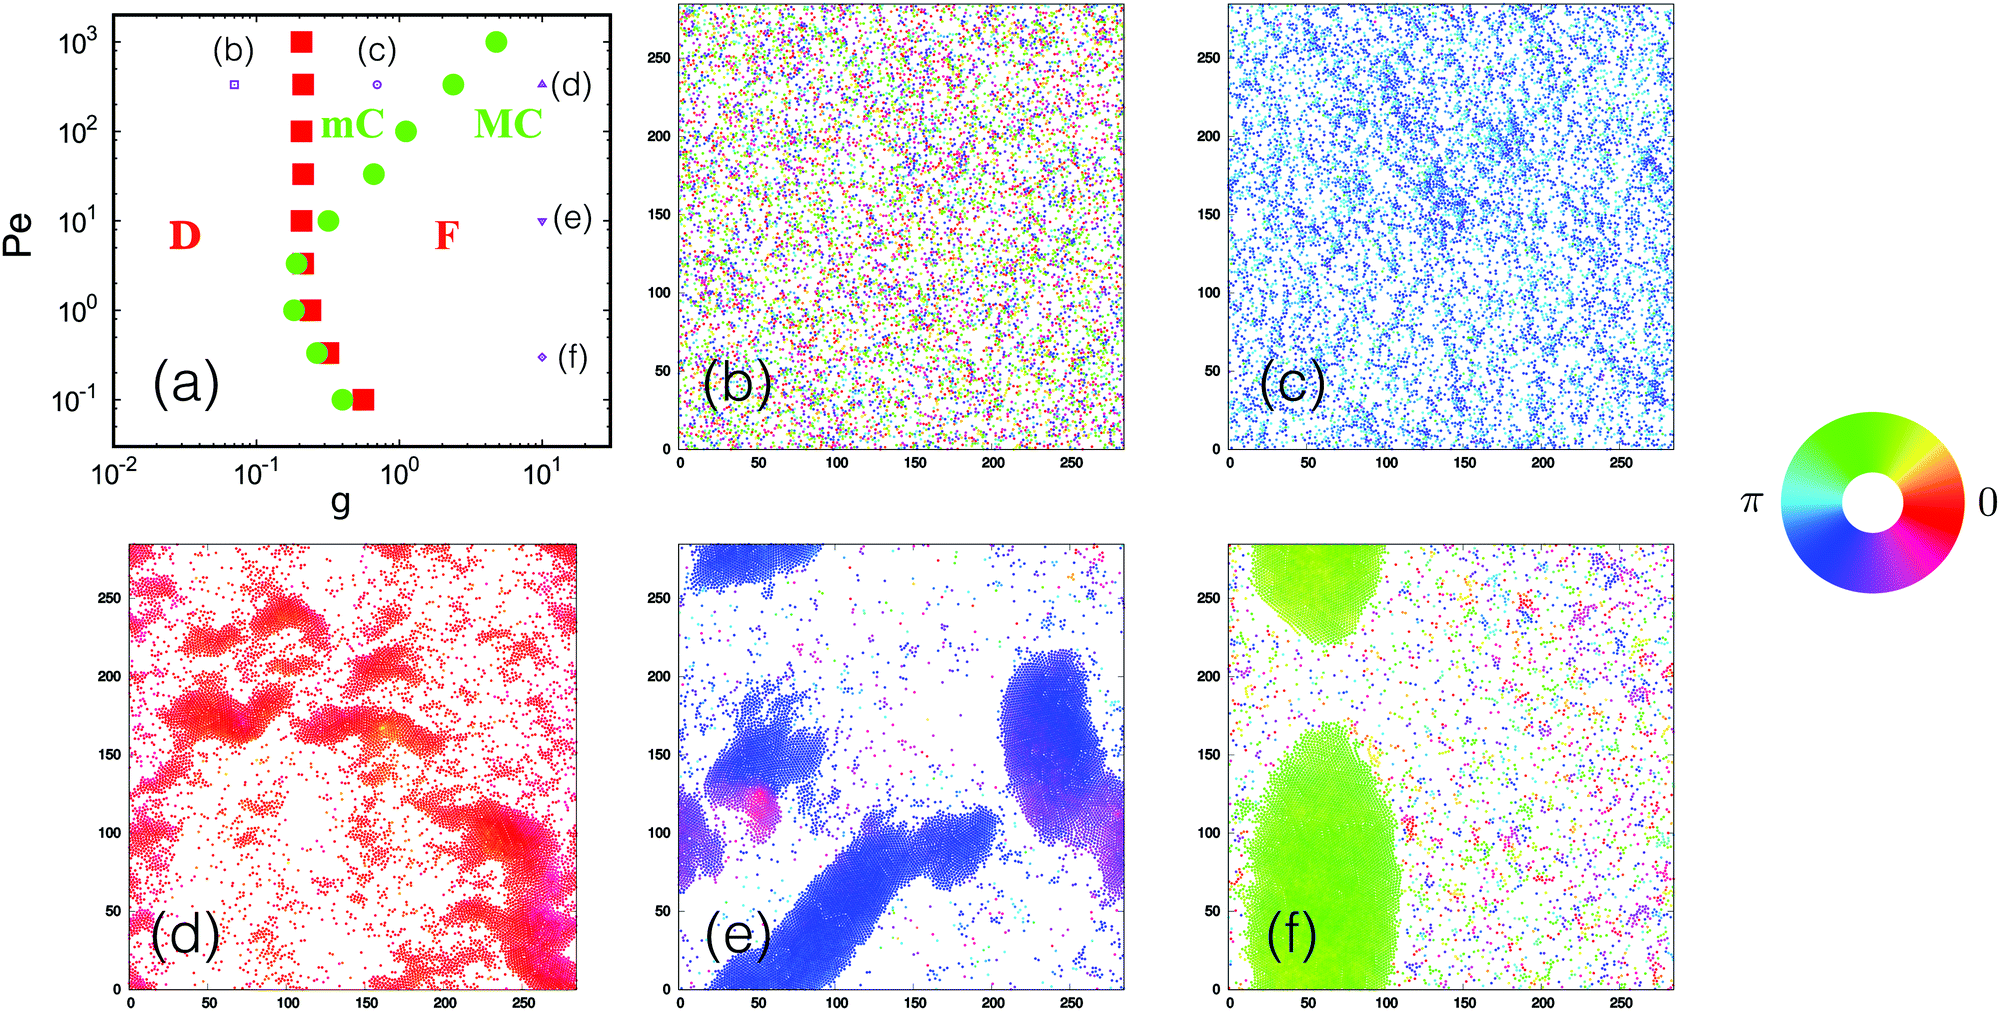
\includegraphics[width=\textwidth]{martin_phaseseparation.png}
		\caption{\parencite{martin-gomez_collective_2018}}
		\label{fig:martin_flocking1}
	\end{figure}
	
	After noting that the phase transition happens with increasing $g$ for any $\mathrm{Pe} > 1$, authors focus on studying this transition in $g$, in the  spirit of an equilibrium phase transition, with $P$ as the order parameter and its susceptibility $\chi = N(\langle P^2 \rangle - \langle P \rangle^2)$. The behavior of the two quantities is similar to what is expected in a continuous phase transition with the critical coupling $g^c = 0.21 \pm 0.02$ (Figure \ref{fig:martin_flocking3}(a)).
	
	In the next part authors focus on clustering phenomena, noting that the cluster size distribution decays exponentially for $g < g*$ and algebraically for $g > g*$. This defines the two phases of microscopic and macroscopic clustering.
	Introducing two new order parameters
	\[ P_x = \left\langle \left| \frac{1}{N} \sum_{i=1}^N \cos(\theta_i) \right| \right\rangle ; \quad
	P_y = \left\langle \left| \frac{1}{N} \sum_{i=1}^N \sin(\theta_i) \right| \right\rangle,
 \]
 it is possible to distinguish between lane-like and band-like behavior in aligned clusters.
 
 \begin{figure}[htp]
	 	\centering
	 	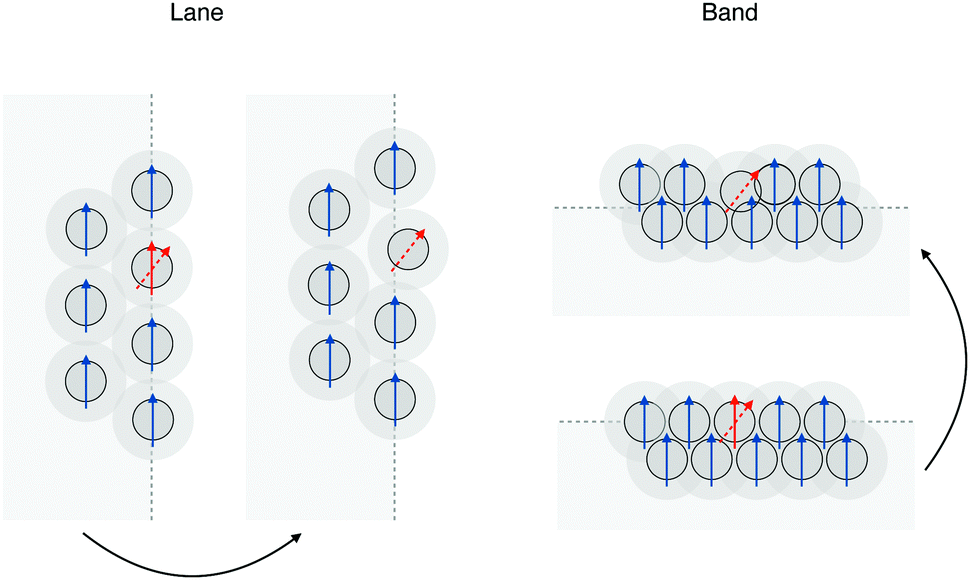
\includegraphics[width=\singfigwidth]{martin_laneband.png}
	 	\caption{\parencite{martin-gomez_collective_2018}}
	 	\label{fig:martin_flocking2}
 \end{figure}
 
 The authors use the radial distribution function 
 \[ g(r) = \frac{1}{N} \left\langle \sum_{j \neq i} \sum_{i} \delta \left( r - |\mathbf{r}_i - \mathbf{r}_j| \right) \right\rangle
 \]
	to characterize the global structure of the largest cluster. Increasing the coupling $g$ at fixed Péclet number makes the peaks higher and shifts them to larger distances, showing that the system is developing a longer range order.
	
	\begin{figure}[htp]
		\centering
		\subfloat[][Polarization and its susceptibility]{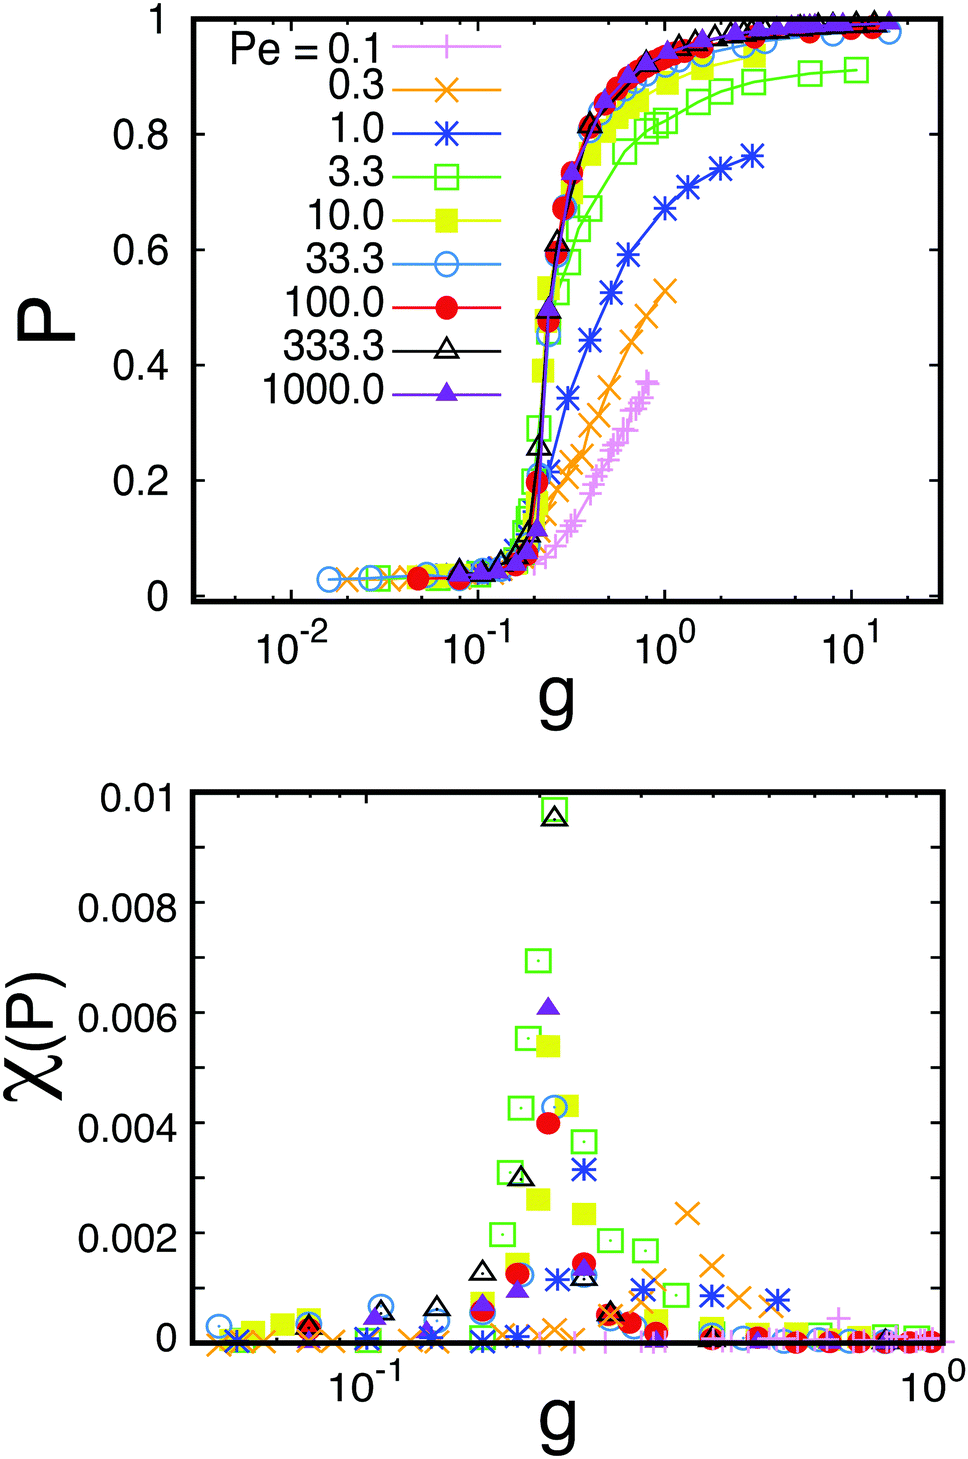
\includegraphics[width=\subfigwidth]{martin_phasetransition.png}}\quad
  \subfloat[][Pair correlation function and static structure factor]{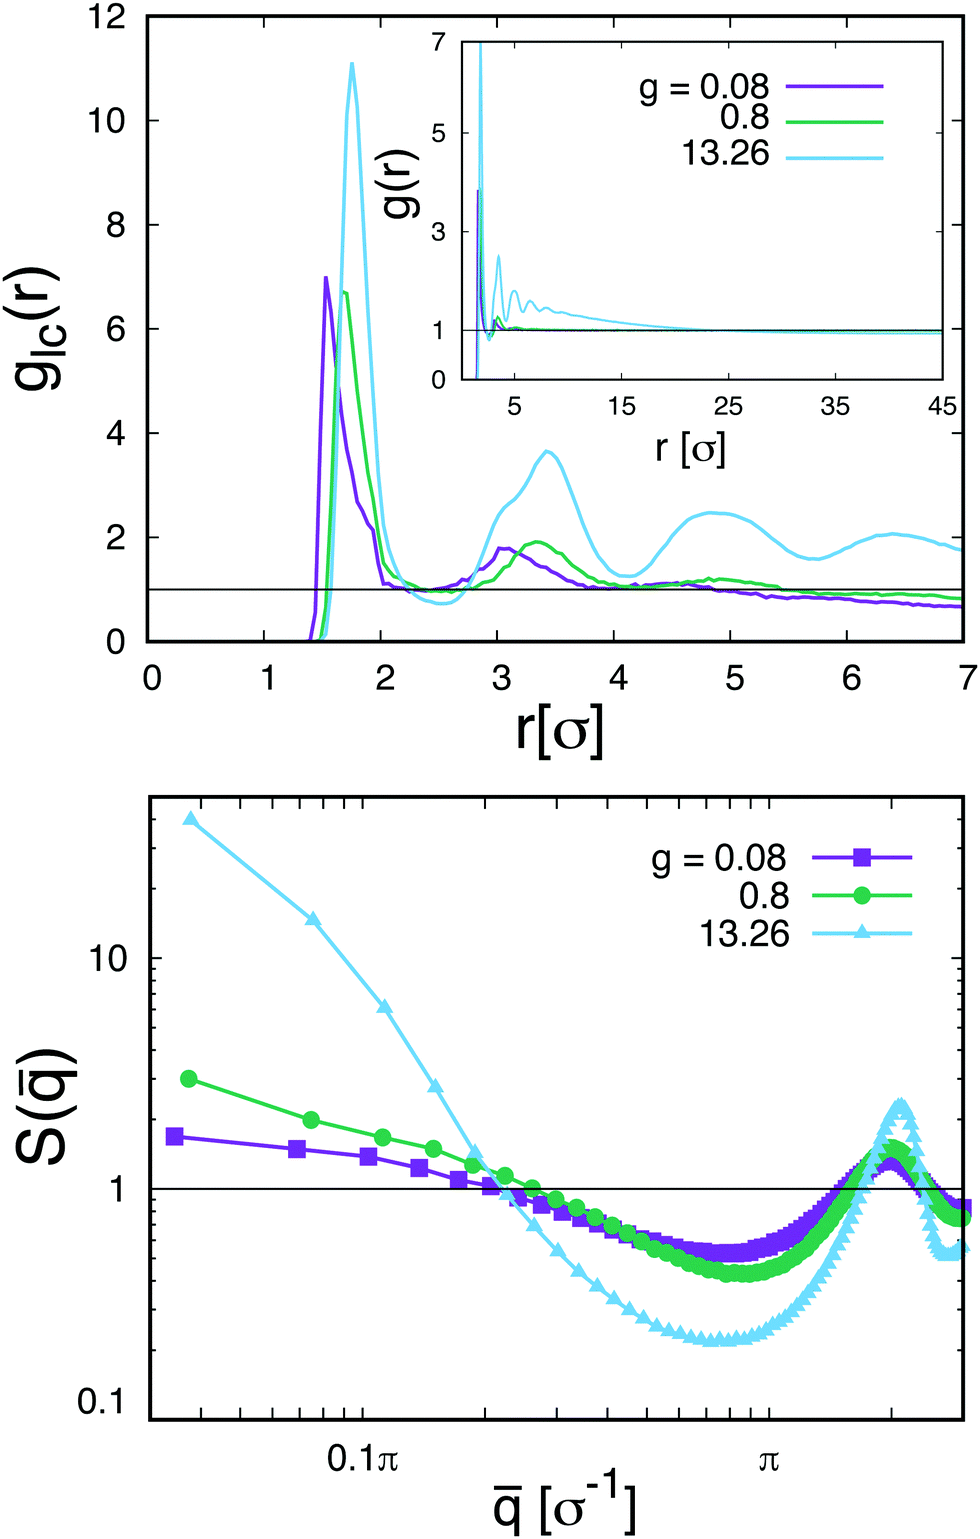
\includegraphics[width=\subfigwidth]{martin_gofr.png}}
 
  \caption{\parencite{martin-gomez_collective_2018}}
  \label{fig:martin_flocking3}
	\end{figure}
	
	In \parencite{caprini_spontaneous_2020}, authors investigate the alignment of instantaneous velocities in cases where motility-induced phase separation occurs. Most literature focuses on the effect that a central 2-body potential, or an explicit aligning interaction which couples the orientational degrees of freedom of single particles, has on the system, but the interplay between phase separation of particles systems and alignment in their velocity has hardly been studied.
	
	In the aforementioned paper, it is shown how, when ABPs systems with a simple repulsive only Weeks-Chandler-Andersen potential phase-separate in a cluster, their velocity tend to form aligned domains, regardless the self propulsion orientation. For this reason, the global polarization is not a good order parameter, even when the computation is restricted to clusters, thus the authors introduce the spatial correlation function of the velocity orientation $Q_i(r) = 1-2\sum_{j} \frac{d{ij}}{\mathcal{N}_k \pi } $, being $d_{ij} = \mathrm{min}\left[|\theta_i - \theta_j|, 2 \pi - |\theta_i - \theta_j| \right]$ the angular distance between two particles and $\mathcal{N}_k$ is the number of particles in a circular shell around the i-th particle, taken with a thickness $\bar{r} = \mathrm{argmax} \{g(r)\}$, and mean radius $k\bar{r}$ with integer $k$. 
	
	It is possible to derive an order parameter from $Q(R)$ integrating it
	\[ 
	R = \int Q(r) dr \]
	where the integral is performed on the cluster domain when present. 
	This seems to be a good order parameter: varying the reorientation time $1/D_r$, $R$ is discontinuous at the point where the MIPS occurs and the result is consistent with established MIPS order parameters as shown in Figure \ref{fig:caprini1}.
	
	\begin{figure}[htp]
		\centering
		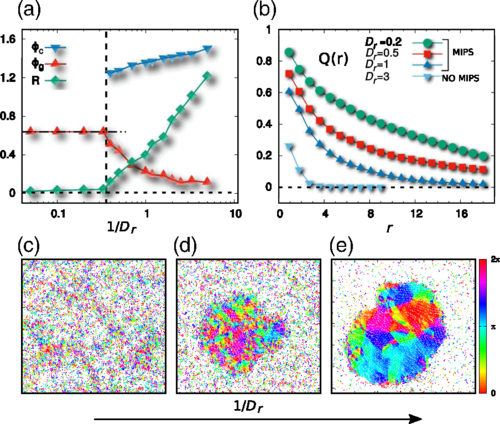
\includegraphics[width=\textwidth]{caprini2.png}
		\caption{\parencite{caprini_spontaneous_2020}}
		\label{fig:caprini1}
	\end{figure}
	
	Going on, the article shows analitically how it is possible to rewrite the equation of motion for the velocity: considering the symmetry in the hexagonal lattice which the particles arrange into, such equation involves a term which depends on the difference between particle's velocity and average velocity of the six surrounding it, thus re-obtaining a Vicsek-like model without a specific aligning interaction.
	
	Some of the first papers cited in this section focus on animal behavior; it is believed that to better represent animal collective motion one have to implement some kind of vision in the model. \parencite{negi_emergent_2022} does so, with an aligning interaction similar to the one in \parencite{martin-gomez_collective_2018}, with the difference that the total torque on particle $i$ is calculated taking into account only particles in the \emph{vision cone} of particle $i$, i.e.\ a circular sector with center of mass of $i$ as center as shown in Figure \ref{fig:negi_vision1}, with a given aperture angle and radius. This is useful to see what happens when \emph{nonreciprocal} interactions, i.e.\ particle $i$ feels the effect of particle $j$ but the vice versa is not true.
	
	\begin{figure}[htp]
		\centering
		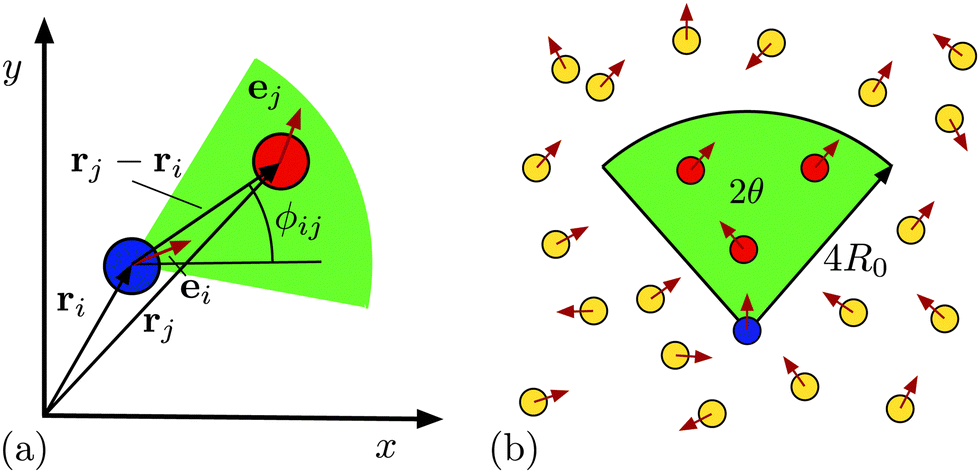
\includegraphics[width=\singfigwidth]{negi_vision1.png}
		\caption{\parencite{negi_emergent_2022}}
		\label{fig:negi_vision1}
	\end{figure}
	
	
	Authors use some tools, such as cluster size distribution, Mean Square Displacement (MSD) and velocity correlation function to study the properties of a collection of \emph{intelligent} ABPs, but they also display some snapshot of the particles' simulation, which are particularly interesting to see what \emph{can} happen when an interaction is acting on the system, both at small and large packing fraction. 
	
	\begin{figure}[htp]
		\centering
		\subfloat[][Low packing fraction]{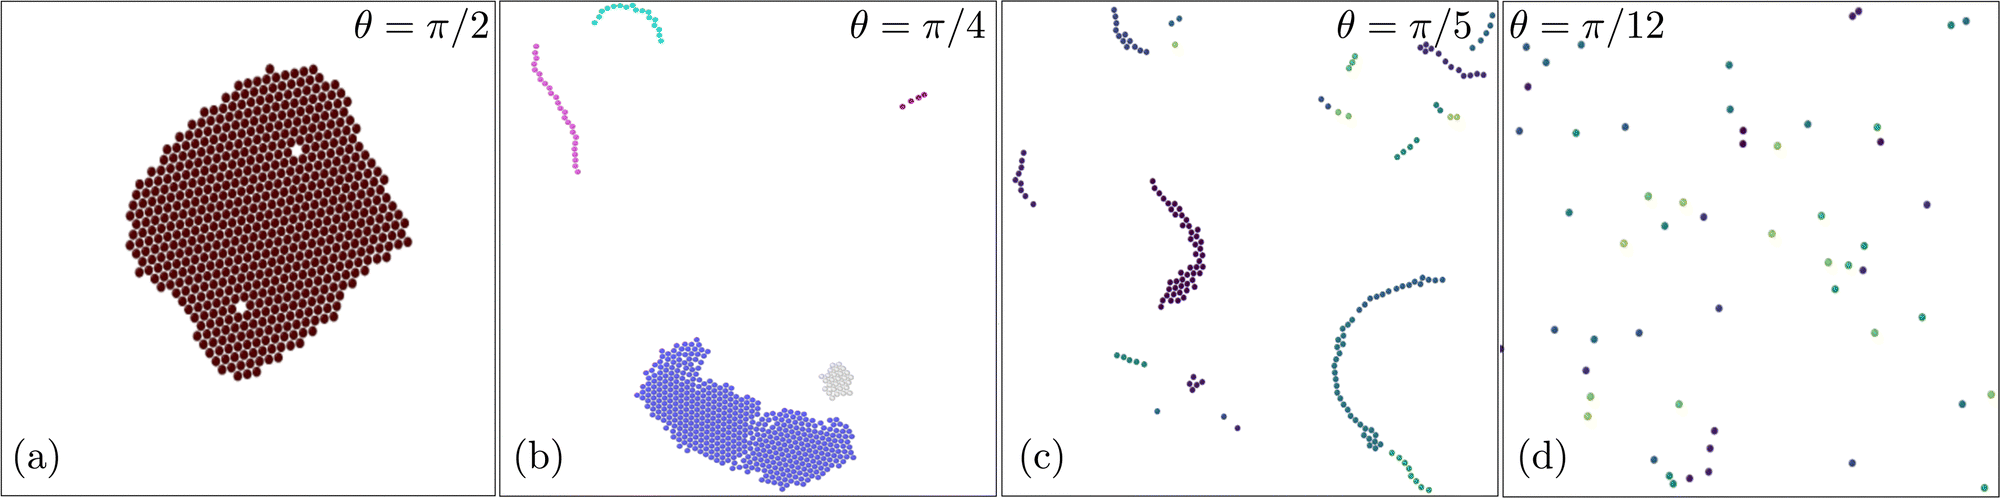
\includegraphics[width=\singfigwidth]{negi_vision2.png}} \\
		\subfloat[][High packing fraction]{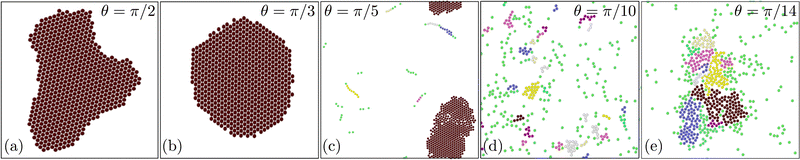
\includegraphics[width=\singfigwidth]{negi_vision3.png}}
		\caption{\parencite{negi_emergent_2022}}
		\label{fig:negi_vision2}
	\end{figure}
	
	\subsection{Analysis of ABPs behavior in experiments}
	There exists quite a large literature that delves into experiments involving active Brownian particles. \parencite{singh_pair_2024} analyzes what happens when two \ch{SiO2-Pt} Janus Particles come together in different configurations; authors take into account hydrodynamics and chemistry involved in the process, classifying the different possible cases. Although here we are trying to build a dry active matter simulation -means, absence of hydrodynamic and medium behavior is not simulated-papers like this accurately describe the phenomenology of these close encounters, which is essential to build minimal models that mimic real-world behavior. The main fact, supported both by simulations and experimental evidence, we can use is that particles do not long-range reorientation due to hydrodynamic or chemical interaction, and that the leading interactions are steric and near-contact chemical. 
	
	Dispersing Janus colloids in a \ch{H2O2} solution in a quasi-2D environment, the types of configurations particles can scatter in are limited and categorized by the authors in four dynamical states. The classification of both approach and departure states, along with a relative frequency histogram is in \ref{fig:singh_pair1}.
	
	\begin{figure}[htp]
		\centering
		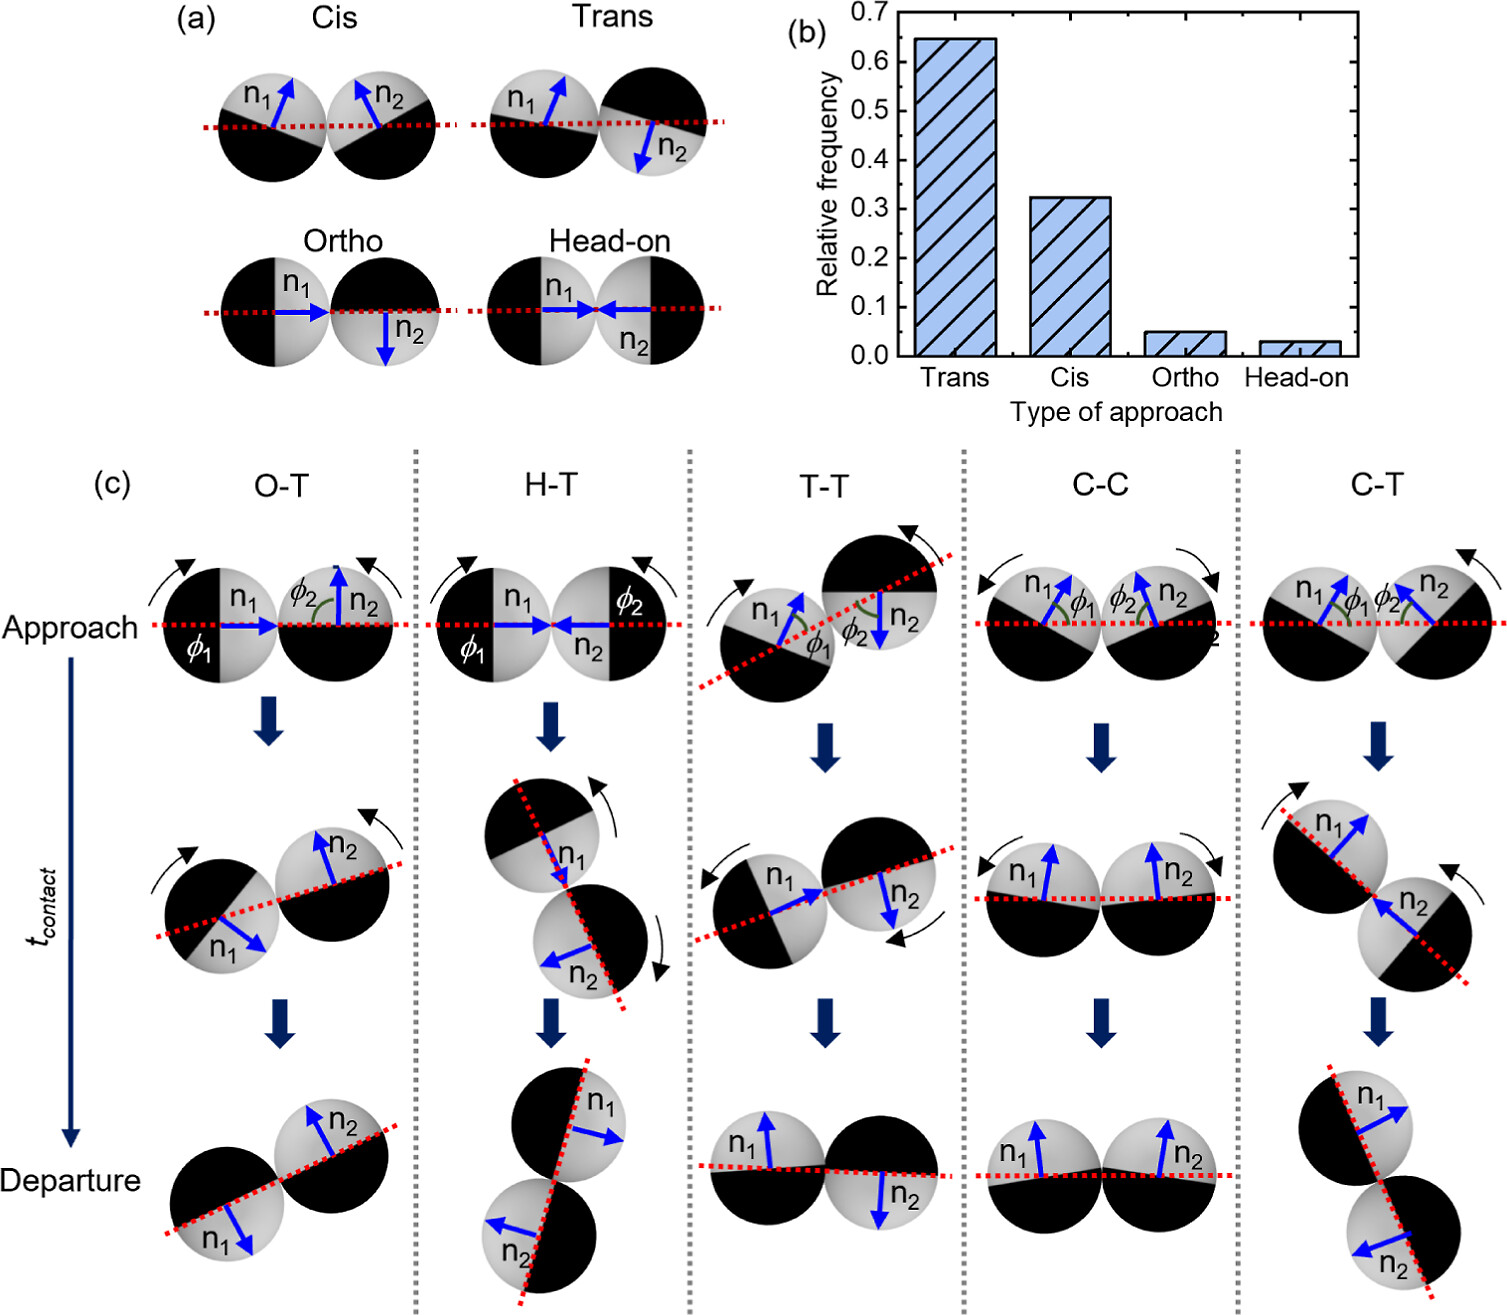
\includegraphics[width=\singfigwidth]{singh_pair1.jpeg}
		\caption{\parencite{singh_pair_2024}}
		\label{fig:singh_pair1}
	\end{figure}
	
	It is evident from this article that particles exert a torque on each other at short range and this interaction, which is a product of the intrinsic asymmetry of a Janus colloid, must be considered in order to capture all the dynamics of these microswimmers.
		
	Emergent properties and collective behaviors might seem a purely theoretic matter but, as was displayed at the start of this section, there are some attempts to challenge this subject from an observational point of view. \cite{maity_spontaneous_2023} aims at doing exactly so, investigating what happens with a double population of active colloidal particles. Those colloids move due to a different mechanism than the one seen before, whose details won't be discussed here, called Quincke instability; with enough particle density, the solvent mediates an aligning interaction which makes the system undergo a Vicsek-like flocking transition that, within a circular confinement, takes place as a vortex motion. The two populations are distinguished by a difference in diameter and in velocity. In the space of some minutes, the initially uniform sample demixes spontaneously, directing to a segregated state where the two populations are well separated and their relative densities have a different radial profile, as shown in Figure \ref{fig:maity1}.
	
	\begin{figure}[htp]
		\centering
		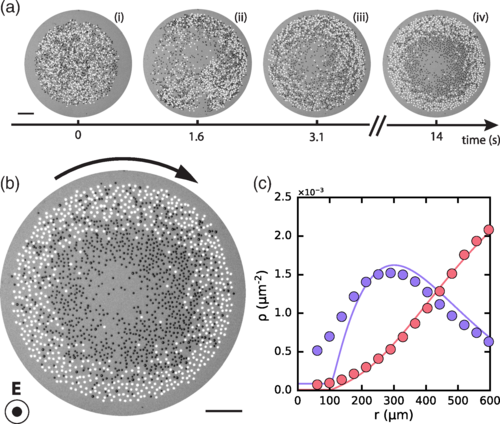
\includegraphics[width=\singfigwidth]{maity1.png}
		\caption{\parencite{maity_spontaneous_2023}}
		\label{fig:maity1}
	\end{figure}
	
	\citeauthor{ostapenko_curvature-guided_2018}, in \cite{ostapenko_curvature-guided_2018} look into the dynamics of real micro swimmers in a confinement. Authors tracked the movements of a single \emph{Chlamydomonas reinhardtii} algae cell within a round and elliptical space. At the same time, they performed a simulation of the algae behavior as an ABP; to better model the dynamics, the alga's placeholder was a dumbbell shaped particle made of two attached spheres of different radius. In the simulation, the steric interaction with the wall was modeled as a Weeks-Chandler-Andersen potential and a torque reorienting the particle near the wall was inserted too.
	
	For different circular confinement radii the radial probability density $P(r)$ was extracted, resulting in a striking agreement between simulations and experiments, as shown in Figure \ref{fig:ostapenko1}.
	\begin{figure}[htp]
		\centering
		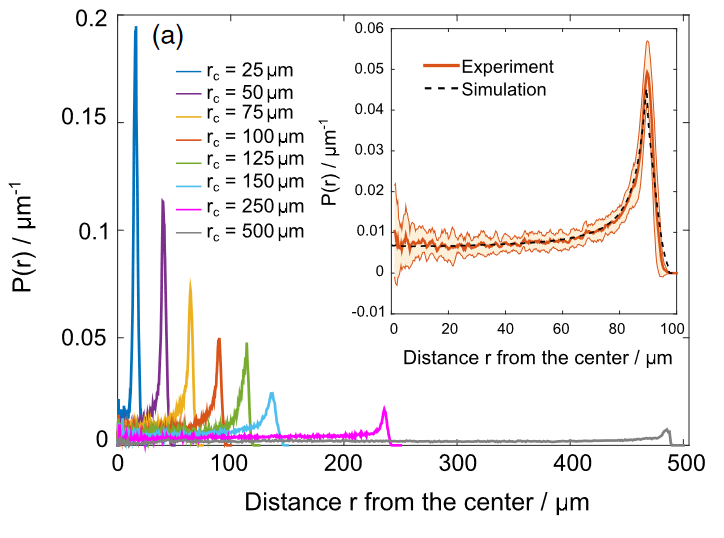
\includegraphics[width=\singfigwidth]{ostapenko1.png}
		\caption{\parencite{ostapenko_curvature-guided_2018}}
		\label{fig:ostapenko1}
	\end{figure}
	
	Next, \citeauthor{ostapenko_curvature-guided_2018} focus on how the swimming statistics depend on the radius of curvature. In order to do so, keeping the results independent from confinement size, simulations and experiments were performed within an elliptical chamber, with the result that the alga spent more time near the walls with the smaller curvature radius. The result is that near-wall swimming probability increases monotonically with the curvature (or decreases monotonically with the radius), and once again, there is a good agreement between experimental data and simulations.
	\begin{figure}[htp]
		\centering
		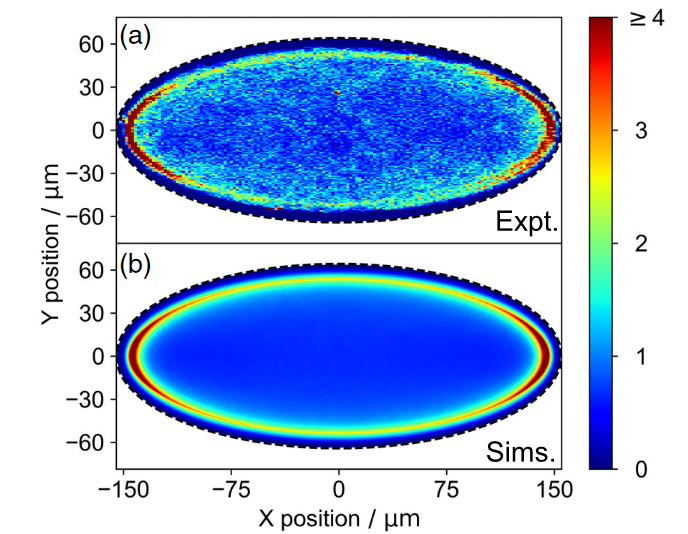
\includegraphics[width=\singfigwidth]{ostapenko2.png}
		\caption{\parencite{ostapenko_curvature-guided_2018}}
		\label{fig:ostapenko2}
	\end{figure}
	
	\subsection{Inference and Machine Learning}
	The matter of inferring interaction potentials starting from simulated data is a complicated one and many techniques can be applied to tackle it. Since the real interactions that occur between a pair of colloidal particles are mostly unknown and in principle may involve chemical gradients, hydrodynamics, electromagnetism and all kinds of interplay between these and other mechanisms, it would be extremely useful to have a tool that predicts forces between particles mapping them in terms of some kind of minimal model e.g.\ a simple central potential. Here, we will focus only on Deep Learning since that is what is used in this work. 
	
	In terms of machine learning model, the simplest approach is using some global attribute of the ABPs ensemble to predict the potential via a Deep Neural Network. \cite{bag_interaction_2021} aims at doing exactly that, exploiting a fact from statistical and matter physics; as authors claim, they use a theorem saying that \enquote{for the fluids with only pairwise interaction (quantum or classical), the pair potential $V(r)$ that leads to a specific $g(r)$ is unique} and the question of predicting which $V(r)$ causes a specific structural correlation like $g(r)$ or, equivalently, $S(q)$ \enquote{is a well defined one}. 
	
	Authors simulated both passive and active Brownian particles to see de difference between equilibrium and non-equilibrium configurations. All the tested potential were of the form $V(r_{ij}) = 4\varepsilon \left[ \left( \frac{\sigma}{r_{ij}} \right)^a - \lambda \left( \frac{\sigma}{r_{ij}} \right)^b \right]
	$ with different values of the parameters. Letting the system reach steady state and then taking $100$ snapshots of the pair correlation function to train the network, the authors show pretty good results regarding the accordance between predicted and real potentials in all the possible phases: gas-like, crystal and liquid-like. (\ref{fig:bag1})
	\begin{figure}[htp]
		\centering
		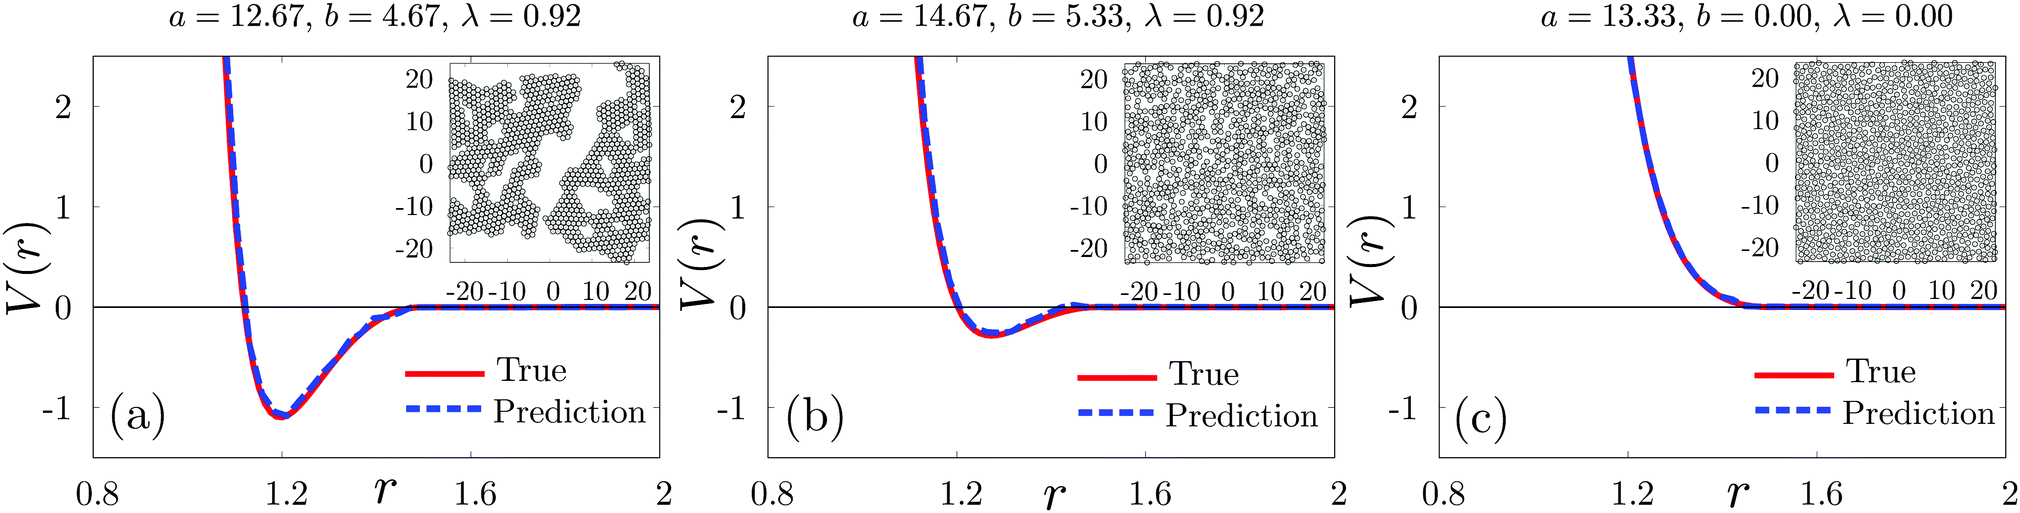
\includegraphics[width=\singfigwidth]{bag1.png}
		\caption{\parencite{bag_interaction_2021}}
		\label{fig:bag1}
	\end{figure}
	
	The non-equilibrium case is a different matter: as soon as self-propulsion is involved, phenomena like MIPS start to occur, pushing the system to cluster. Some literature has introduced effective many-body attractive potential to explain the change in structure caused by particles' motility, even in cases where just an explicit repulsion is present, and the results presented by \citeauthor{bag_interaction_2021} seem to point in that direction as well. 
 	\begin{figure}[htp]
		\centering
		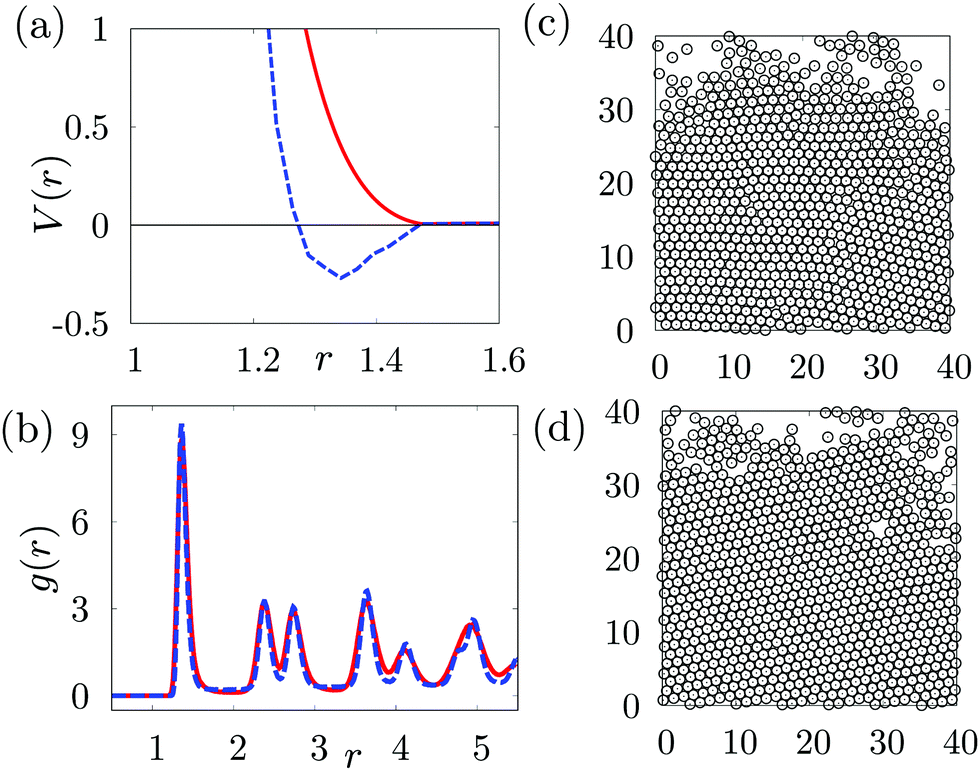
\includegraphics[width=\singfigwidth]{bag2.png}
		\caption{\parencite{bag_interaction_2021}}
		\label{fig:bag2}
	\end{figure}
	As Figure \ref{fig:bag2}(b) shows, pair correlation functions in the case of active repulsive particles is similar to that of passive attractive particles, since only structure-meaning: particles' positions-is involved, tricking the network into predicting an attractive potential. This is a good result in simulation context and sheds light on some theoretical statements, nonetheless this approach does not fit the objective of present thesis project, which tries to obtain \emph{actual} 2-body interactions in ABPs systems. 
	
	An alternative approach is working directly on positions and velocities of single particles. It is an accepted fact that the best way to make AI learn something about a problem is taking the invariances and symmetries of said problem are taken in to account in the model design. The most efficient way to store information about a set of interacting bodies is a graph, where vertices represent single body information like position, velocity, mass or charge and edges contain information about the potential that make pairs of particles communicate. With these facts in mind, it is clear why Graph Neural Networks (GNNs or GNs) are so popular in several fields of physics. The distinction between GNNs and GNs is that the first one is a term that represent every kind on Neural Networks related with graphs, regardless the structure, while the Graph Network framework represents a specific network with a graph structure. An actual GN is actually a container, structured as a graph, which in principle holds three networks or functions, or models: one is the edge function $\phi^e$, which predicts edge features, a node function $\phi^v$ which predicts single nodes features and a global function $\phi^u$ that works in the same fashion. $\phi^e$ maps from a pair of nodes and some information stored on the edge to a message vector which lies in the \emph{latent space}. Then, all the messages from sending nodes into a receiving one  are aggregated by means of a permutation-invariant function, namely sum, mean, max etc.; the node model $\phi^v$ takes the aggregated messages along with the node information and predicts some feature. Finally, a global function gathers all the information and predicts a global attribute \cite{battaglia_relational_2018}.
	
	In the case of interacting bodies, edge function works as the force law and node function plays the role of the second Newton's law, calculating the resulting force and applying it to obtain particle's acceleration. In \cite{cranmer_discovering_2020} there is the application of this kind of approach in the case of Newtonian dynamics (along with Hamiltonian dynamics and a Dark Matter simulation, which we will not focus on) of a set of particles with interactions among them. After simulating the dynamics of a set of interacting bodies with several kinds of interaction forces, \citeauthor{cranmer_discovering_2020} experiment with different message dimensionalities. This theme causes doubts when working with GNs and multiple strategies can be explored, the most natural of them is creating a bottleneck using the dimension of the problem, e.g.~if particles move in N dimensions than forces are N-D and one (especially a physicist) may be tempted to think that, since messages should represent forces, this is the best dimensionality to use; the other approach is using a high-dimensional message, e.g.~100D, in training and then selecting the N most meaningful dimensions to plot the force in N-D. \citeauthor{cranmer_discovering_2020} try both of these strategies as well as a hybrid one: instead of implementing a hard bottleneck, they let the network learn with a 100D message but with regularization terms that encourage the model to learn compact representations of the forces, in accordance with an Occam's razor type of reasoning. Doing this, message is still 100-dimensional, but now most of its components have no variability, leaving few of them with some information stored. Results show that, although an explicit bottleneck works well, the best performing strategy is the $L_1$ regularization. The whole workflow is explained in Figure \ref{fig:cranmer1}.
	
	 \begin{figure}[htp]
		\centering
		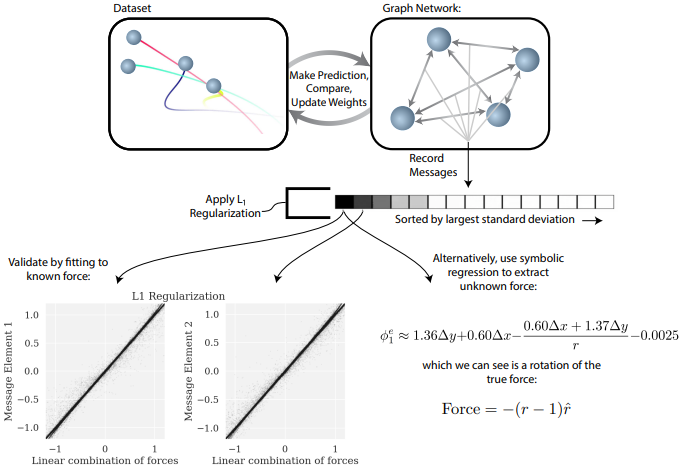
\includegraphics[width=\singfigwidth]{cranmer1.png}
		\caption{\parencite{cranmer_discovering_2020}}
		\label{fig:cranmer1}
	\end{figure}
	
	Since all the operations that happen inside the node function are linear, it is evident that the message components will be some kind of linear combination of the actual forces. After letting the network train, one can search for the linear operation that minimizes the difference between the learned message components and the forces. 
	
	An alternative way of extracting the forces is using symbolic regression, which will give some insights about the functional form of the interaction potential. The modeling engine used is \emph{eureqa}, and the best model is selected between several candidates at different complexity levels, choosing a more complicated one only when it is worth it.
	
	A real application to active Brownian particles can use some of the already seen tactics, but it requires some tweaks with respect to the Newtonian dynamics approach. The most important change is in the physics: in a system without inertia, the meaning of acceleration is not clear and there is a linear relation between a force and a velocity. In this framework, \citeauthor{ruiz-garcia_discovering_2024} have developed a variant of the graph network by \citeauthor{cranmer_discovering_2020} that can work with ABPs dynamics, called ActiveNet. In \cite{ruiz-garcia_discovering_2024}, the graph network takes as input positions and orientations of a set of simulated ABPs and tries to predict their velocity, given the instantaneous velocity $\frac{\vec{x}(t + \Delta t) - \vec{x}(t)}{\Delta t}$ as the ground truth. In this case the role of the node function is not only to predict the velocity starting from the sum of the forces, but also of learning and adding to it the self propulsion velocity that drives the particles. This is a useful result, since after predicting the interaction force one can take the output of the node function and subtracting the edge function output in order to understand which part of the velocity can be explained through interaction and which is due to self propulsion.
	A schematic representation of the ActiveNet GN is in Figure \ref{fig:ruiz1}.
	\begin{figure}[htp]
		\centering
		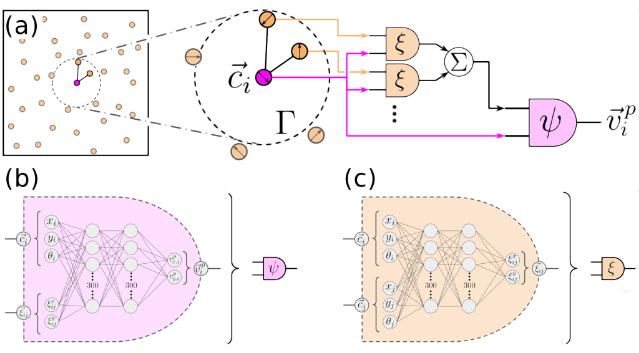
\includegraphics[width=\singfigwidth]{ruiz1.png}
		\caption{\parencite{ruiz-garcia_discovering_2024}}
		\label{fig:ruiz1}
	\end{figure}
	In order to train the network, successive iterations are done, increasing the threshold distance to consider two particles as interacting. At the end of the training, the network gets tested and results show that it works well to predict both the self-propulsive force and the interaction potential. Having an internal way of taking into account the active velocity, this method works better than static structure-based ones, like \cite{bag_interaction_2021}, in out of equilibrium particles ensembles where MIPS takes place, learning a repulsive interaction even though the system is clustered. Clearly, ActiveNet fails at short distance, since very few data are presented. Having Brownian motion at his base, the studied system has an internal degree of randomness. The goal of a machine learning task should be to reduce the loss (difference between ground truth and predictions) to make it as small as the noise. This can be useful to estimate the diffusion coefficient and works well even with few examples, as long as the temperature is high enough. 
	
	An important result of this paper is the application of the method to experimental data. The network needs some adjustments in order to work since experiments have some hurdles that must be overcome. To not be influenced by stuck particles, the network is fed with the bias that forces depend only on distances and not positions. Moreover, self-propulsion is forced to depend only on the orientation of particles. Experimental observations contain thousands of particles and their direction is clearly measurable. Results show some similarities with the expectations but not much can be said since the actual interactions are not known (even though in this case authors used electric fields and some kind of guess can be made about the interactions). Authors claim that probably symbolic regression is needed in order to discover the actual form of the interaction.
	
	\section{Background}
	\subsection{Passive Brownian Motion}

	Before adding the self-propulsion velocity, it is worthwhile to outline some facts about Passive Brownian motion. The first formulation of the theory of Brownian motion was obtained by Albert Einstein in a 1905 paper, where the mean square displacement was given in terms of a linear relation with time, with a diffusion coefficient $D_t$ as $\sqrt{\bar{x}^2} = \sqrt{2D_t t}$. Here, we outline the derivation as it was presented by Paul Langevin some years afterwards, following \cite{gardiner_handbook_2004}.
	
	It is known from statistical mechanics that a Brownian particle in equilibrium will have as mean kinetic energy
	\[ \langle \frac{1}{2}mv^2 \rangle =  \frac{1}{2} k_B T\]
	where $T$ is the absolute temperature and $k_B$ is Boltzmann's constant. If we assume the same formula as in macroscopic hydrodynamics, the viscous drag acting on the particle will be of the form $-6 \pi \eta a \frac{\mathrm{d}x}{\mathrm{d}t}$, being $a$ the particle's radius and $\eta$ the viscosity of the fluid. Due to the random collisions with the fluid molecules, a passive Brownian particle experiences a \emph{fluctuating force} $X$. The equation of motion for the particle is thus
	\[ m \frac{\mathrm{d}^2x}{\mathrm{d}t^2} = -6 \pi \eta a \frac{\mathrm{d}x}{\mathrm{d}t} + X \]
	which we multiply by $x$ getting
	\[ \frac{m}{2} \frac{\mathrm{d}^2}{\mathrm{d}t^2}(x^2) - mv^2  = -3 \pi \eta a \frac{\mathrm{d}(x^2)}{\mathrm{d}t} + Xx \]
	where we called $v = \mathrm{d}x/\mathrm{d}t$. Averaging on the ensemble of particles we have
	\[ \frac{m}{2} \frac{\mathrm{d}^2\langle x^2 \rangle}{\mathrm{d}t^2} + 3 \pi \eta a \frac{\mathrm{d}\langle x^2 \rangle}{\mathrm{d}t} = k_B T \]
	where the value for the mean kinetic energy was plugged in and we averaged the product $Xx$ to zero, being $X$ highly irregular (in modern times we just write everything in terms of a 0 mean Gaussian stochastic process, namely a Wiener process). The general solution to the differential equation for $\langle x^2 \rangle$ is 
	\[ \frac{\mathrm{d}\langle x^2 \rangle}{\mathrm{d}t} = \frac{k_B T}{3 \pi \eta a} + C \exp(-6 \pi \eta a t / m)\]
	with $C$ an arbitrary constant. It is possible to neglect the exponential, since Langevin estimated its characteristic time about $10^{-8}$ s, and then integrate to get the equation
	\[ \langle x^2 \rangle - \langle x_0^2 \rangle = \frac{k_B T}{3 \pi \eta a}t\]
	which corresponds to what Einstein found out if $D_t \equiv k_B T/(6 \pi \eta a)$.
	
    Adapting this framework to our case-study, where the particle's orientation is considered, we need to take in to account both random forces and torques so that its motion is purely diffusive, both in position and orientation with the following diffusion coefficients
	\begin{equation}
		D_t = \frac{k_B T}{\gamma_t} \quad D_r = \frac{k_B T}{\gamma_r} 
	\end{equation}
	
	being $\gamma_t = 6 \pi \eta a$ and $\gamma_r = 8 \pi \eta a^3$  the respective drag coefficients, where $a$ is the particle radius and $\eta$ is the fluid viscosity. The basis to build the model upon is the Langevin equation
	
	\begin{equation} \label{eq:lang1}
		m \mathbf{\ddot{r}} = -\gamma_t \mathbf{\dot{r}} + \mathbf{F}_{th}
	\end{equation} 
	where $\mathbf{F}_{th}$ is the random force given by the collisions with the fluid molecules.
	
	Given that a typical Brownian particle will have a characteristic body-length in the order of $ \mathrm{\sim\mu m}$ and a velocity of $\sim\mu \mathrm{m s}^{-1}$ the system can be studied in low-Reynolds number regime being 
	\[Re = \frac{\rho v a}{\eta} \sim 10^{-6} \]  
	where $\rho$ is the fluid density, $v$ is the particle speed, $a$ is the particle radius and $\eta$ is the fluid viscosity and the values of density and viscosity for water were plugged in. As a consequence of this fact, inertial effects can be neglected and it is possible to study the system in the \emph{overdamped} regime, turning the Langevin equation \ref{eq:lang1} into
	\begin{equation} \label{eq:lang2}
		\gamma_t \mathbf{\dot{r}} = \mathbf{F}_{th}
	\end{equation}
	which can be rewritten as:
	\begin{equation}
		\mathbf{\dot{r}} = \sqrt{2D_t}\mathrm{d}\mathbf{W}
	\end{equation}
	where $\mathrm{d}\mathbf{W}$ is the derivative of a zero mean, variance 1 Wiener process.
	In a homogeneous environment, rotational and translational motions are independent from each other, so that the equations of motion for a passive Brownian particle are
	
	\begin{equation}
		\dot{x} = \sqrt{2D_t}dW_x, \quad \dot{y} = \sqrt{2D_t}\mathrm{d}W_y, \quad \dot{\theta} = \sqrt{2D_r}\mathrm{d}W_{\theta}
	\end{equation}
	
	%Ornstein and Uhlenbeck, in a 1930 paper \citeauthor{uhlenbeck_theory_1930}, outlined all the statistical properties of Brownian motion, including the mean square displacement, which in 2 dimension read $\text{MSD}(\tau) = 4D_t \tau + \frac{4k_B T}{m} \tau_m^2 \left[e^{-\tau/\tau_m} - 1\right]$.
	
	\subsection[ABP simulations]{Physics and Numerical Simulations of ABPs}
		Despite the variety in single agent properties and self-propulsion mechanisms, it is possible to identify some key features that are shared between all ABP systems. The most important characteristic of an ABP is that, notwithstanding a symmetric shape (often in literature, and always in this work, spherical), each particle has a preferred axis which lies along the direction of self-propulsion.
		
		With this hypothesis, rotational diffusion has now become relevant since the direction of self-propulsion varies randomly with a characteristic time scale which corresponds to the inverse of the rotational diffusion coefficient $\tau_r = D_r^{-1}$. 
		
		Adding a constant-magnitude self-propulsion velocity $\mathbf{v}$ into the equations of motion, we get:
		\begin{equation}
			\dot{x} = v \cos{\theta} + \sqrt{2D_t}dW_x , \quad \dot{y} = v \sin{\theta} + \sqrt{2D_t}dW_y, \quad \dot{\theta} = \sqrt{2D_r}dW_{\theta}
		\end{equation}
		where $\theta$ is the particle orientation and $v$ is the magnitude of the self-propulsion velocity.
		
		As a consequence, the resulting finite-differences equations are:
		\begin{equation} \label{eq:fin_diff1}
			\begin{cases}
				x_{n+1} = x_n + v \cos\theta \Delta t + \sqrt{2D_t \Delta t} \, W_{x,n},\\
				y_{n+1} = y_n + v \sin\theta \Delta t + \sqrt{2D_t \Delta t} \, W_{y,n},\\
				\theta_{n+1} = \theta_n + \omega \Delta t + \sqrt{2D_t \Delta t} \, W_{\theta,n}\\
			\end{cases}
		\end{equation}
		where the case of a deterministic self-propulsion angular velocity $\omega$ is also taken into account.
		
		It is possible to insert external forces and torques in the system, where \emph{external} means they are not due to the self-propulsion. Even though in literature there are examples of uniform external potentials, e.g.\ electric and magnetic fields, being applied on the ABP ensemble as a whole, in this work the only external force is the interaction between particles, which is applied in the low-Reynolds number regime as:
		\begin{equation} \label{eq:fin_diff_with_forces}
			\begin{cases}
				x_{n+1} = x_n + \left( v \cos\theta + \frac{D_t}{k_B T} F_{ext,x} \right) \Delta t + \sqrt{2D_t \Delta t} \, W_{x,n},\\
				y_{n+1} = y_n + \left( v \cos\theta + \frac{D_t}{k_B T} F_{ext,y} \right) \Delta t + \sqrt{2D_t \Delta t} \, W_{y,n},\\
				\theta_{n+1} = \theta_n +\left(\omega + \frac{D_r}{k_B T}{}T_{ext}\right) \Delta t + \sqrt{2D_t \Delta t} \, W_{\theta,n}\\
			\end{cases}
		\end{equation}
		where applying a force or a torque just linearly translates to a linear or angular velocity change, with the respective drag coefficients as proportionality constant.
		
		\subsection{Stochastic integration}
		The topic of integrating a stochastic differential equation (SDE) is a fundamental part of present work and an important object of investigation in the physics and mathematics community. The most simple SDE one can write is
		\begin{equation} 
			\mathrm{d}x = f(x)\mathrm{d}t + g(x)\mathrm{d}W 
		\end{equation} 
		where $\mathrm{d}W$ is the increment of a Wiener process $W(t)$, defined by its probability
		\begin{equation} 
			P(W(t)) = \frac{1}{\sqrt{2 \pi t}} e^{-\frac{W(t)^2}{2t}}
		\end{equation}
		in which we assumed 0 mean and no correlation at different times, which reads $\mathrm{d}W = \xi(t)\mathrm{d}t$ with $ \langle \xi(t) \xi(t') \rangle = \delta(t-t')$.
		
		Now, to solve such SDE, we need to compute integrals of the form $\int W \mathrm{d}W$. We start by defining the mean square limit as
		\begin{equation} 
			\text{m.s.} \lim_{n \to \infty} X_n = X \iff \lim_{n \to \infty} \langle(X_n - X)^2\rangle = 0 
		\end{equation}
		where the average $\langle \cdot \rangle$ is taken over different realizations of the stochastic process. With this, the stochastic integral is defined in terms of a discrete sum
		\begin{equation} 
			\int_0^t W \, dW = \text{m.s.} \lim_{n \to \infty} \sum_{i=1}^n W(t_i^*) \left[ W(t_i) - W(t_{i-1}) \right] 
		\end{equation}
		with $t_{i-1} < t_i^* < t_i$, that is better defined in terms of a constant $\alpha$ as $t_{i-1}+\alpha (t_i - t_{i-1})$. Using the increment independence property of the Wiener process, we can compute the sum getting 
		\begin{equation} 
			\sum t_i-1 + \alpha(t_i - t_{i-1}) = \alpha t 
		\end{equation}
		so that the result of the integral depends on $\alpha$. In principle, no value in $[0,1]$ is denied, but in literature only two values are found: $\alpha = 0$, which defines Itô method, and $\alpha = 1/2$, specific for Stratonovich method, which gives the \emph{standard} result that can be obtained through Riemann integration. 
		
		With all of this, we are ready to integrate our SDE, formally
		\begin{equation} 
			x(t) - x(0) = \int_{0}^{t} f(x(s)) \mathrm{d}s + \int_{0}^{t} g(x(s)) \mathrm{d}W
		\end{equation} 
		considering only the second term in the right-hand side, and Taylor-expanding it we get
		\begin{equation} 
			\int_0^t g(x) \, dW \approx \int_0^t dW \, \big[g(x(0)) + g'(x(0))(x(s) - x(0))\big]
		 \end{equation}.
		 
		 The Itô versus Stratonovich controversy poses a subtle but fundamental problem: since $g$ depends on $x$ which depends on $t$, to compute the $i$-th step when we have the $i-1$-th we need to evaluate $g$ at an instant $t_i^*$, subsequent to $t_i$, where the value of $x$ is not known yet, in principle. Only the Itô prescription solves this issue, using the concept of \emph{nonanticipating} functions.
		 
		 With all of this said, it is possible to state that the type of calculus used, i.e.~the value of $\alpha$, is actually a parameter of the model and there is literature showing that the physical quantities obtained through simulations are different if one chooses a method over another \cite{mannella_ito_2012}.	
		
		Let us apply this theoretical notions to the equations for ABPs. Only accounting for $\theta$ and $x$, we have
		\begin{equation} 
			\begin{cases}
			\mathrm{d}x = f_x(x)\mathrm{d}t + v_0\cos(\theta)\mathrm{d}t + \sqrt{2D_t}\mathrm{d}W_x \\
			\mathrm{d}\theta = \sqrt{2D_r}\mathrm{d}W_\theta
			\end{cases} 
		\end{equation} 
		where in $f$ we included all possible interactions a particle can undergo. For now we set that part to 0 since in does not give particular problems and consider only the terms which contain stochastic parts. We integrate to get
		\begin{equation}
			\begin{cases}
				x(h) - x(0) =  \int_{0}^{h}v_0 \cos(\theta(s)) \mathrm{d}s + \int_{0}^{h} \sqrt{2D_t}\mathrm{d}W \\
			\theta(s) - \theta(0) \sim \sqrt{2D_r s} \sim o(\sqrt{s})
		    \end{cases}  
	    \end{equation}
		being $\int_{0}^{s}\mathrm{d}W = \sqrt{s} y_1$ with $y_1 \sim \mathcal{N}(0,1)$. We plug what obtained for $\theta$ in the first order Taylor expansion of cosine to get ($\theta_x \equiv \theta(x)$ for short)
		\begin{align} 
			x(h) - x(0) &=  \int_{0}^{h}v_0 \left[\cos(\theta_0) - \sin(\theta_0)(\theta_s-\theta_0)\right]\mathrm{d}s + \int_{0}^{h} \sqrt{2D_t}\mathrm{d}W  \\
			& = \sqrt{2D_th} z_1 + hv_0 \cos\theta_0 - \sin \theta_0 y_1 \sqrt{h} \int_{0}^{h}\mathrm{d}s
	    \end{align}
	    with $z_1 \sim \mathcal{N}(0,1)$, and we notice that the last term is $o(h^{3/2})$, leaving us with the first order.
	    
	    This makes what we saw for the finite difference equations correct.
	    
		\subsection{Algorithms}
		
		
		\begin{algorithm}
			\caption{The simulation algorithm} \label{alg:sim1}	
			\begin{algorithmic}[1]
				\For{i in particles in ensemble}
				\State{$ \vec{r}_{i}\gets \vec{r}_{i,0} $}\Comment{position $\vec{r}_{i,0}$ is randomly initialized in the simulation space}
				\State{$\theta_{i}\gets \theta_{i,0}$}\Comment {$\theta_{i,0} \sim \mathrm{Uniform}([0, 2\pi])$}
				\State{$v\gets v_0$}\Comment{Can be initialized as a constant or a random variable}
				\EndFor
				\For{n in timesteps}
				\For{i in particles in ensemble}
				\State{$\vec{F}_{i,n} = \sum_{j}^{Np}{\vec{F}_{ij,n}}$}
				\State{$w_{i,n} \sim \mathcal{N}(0, \sqrt{2D_t \Delta t})$}
				\State{$z_{i,n} \sim \mathcal{N}(0, \sqrt{2D_r \Delta t})$}
				\State{$ \vec{r}_{i,n+1}\gets \vec{r_n} + w_{i,n} + v (\cos\theta_{i,n}, \sin\theta_{i,n})\Delta t + \vec{F}_{i,n}\Delta t / \gamma _t $}
				\State{$\theta_{i,n+1}\gets \theta_{i,n} + z_{i,n} + \omega_{i,n} \Delta t + T_{i,n} \Delta t/\gamma _r$}
				\EndFor
				\EndFor
			\end{algorithmic}
		\end{algorithm}
		

\end{document}